%!TEX root = ../GLUTthesis.tex

%为了便于查找和修改,还可以拆分文件为子章节,并通过input导入。


\section{模板结构}

模板文件的结构,如下表所示:
\begin{table}[ht]\centering
\begin{tabular}{r|l|l}
	\hline
	\multicolumn{2}{l|}{GLUTthesis.tex }  & 主文档,在其中填写正文  \\ \hline
content 文件夹 & info.tex  & 论文信息  \\ \cline{2-3} \hline
content 文件夹 & abstractcn.tex & 中文摘要、关键词  \\ \hline
content 文件夹 & abstracten.tex & 英文摘要、关键词  \\ \hline
content 文件夹 & content.tex & 正文  \\ \hline
content 文件夹 &  thanks.tex & 致谢  \\ \hline
content 文件夹 & additional.tex & 附录  \\ \hline
	\multicolumn{2}{l|}{images 文件夹}                  & 存放图片文件.                   \\ \hline
	\multicolumn{2}{l|}{GLUTthesis.cls}             & 定义文档格式的 class file,不可删除 \\ \hline
	\multicolumn{2}{l|}{GLUTthesis.bib}             & 参考文献存放 \\ \hline
	\multicolumn{2}{l|}{gbt7714.sty}             & 参考文献格式,不可删除 \\ \hline
	\multicolumn{2}{l|}{gbt7714-unsrt.bst}             & 参考文献格式,不可删除 \\ \hline
\end{tabular}
\end{table}

无需也不要改变、移动上述文档的位置。

 \subsection{使用步骤}

1、进入 content 文件夹,  打开 info.tex 填写论文相关信息;
打开 abstractcn.tex、abstracten.tex 这两个文档,分别填写中、英文摘要、关键词;打开 thanks.tex 填写致谢;打开 content.tex 填写正文部分;打开 addtional.tex 填写附录内容。

2、将图片放入 images 文件夹。

3、将参考文献信息录入 GLUTthesis.bib,并在正文中正确引用。

4、使用 XeLaTeX 编译。具体见 \ref{sec-compile} 节。



\subsection{编译方法} \label{sec-compile}

使用 XeLaTeX 编译,直接生成~pdf 文件。


\subsection{其他}
\subsubsection{其他1}
无。
\subsubsection{其他2}
无。
\newpage 


%%%%%%%%%%%%%%%%%%%%%%%%%%%%%%%%%%%%%%%%%%%%%%%%%%
\section{字体操作}
\subsection{字体调节}

\begin{tabular}{ll}
	\verb|\songti|   & {\songti 宋体}   \\
	\verb|\bfseries|    & {\bfseries 粗宋体}    \\
	\verb|\sffamily| & {\sffamily 黑体} \\
	\verb|\bfseries\sffamily| & {\bfseries\sffamily 粗黑体} \\
  \verb|\ttfamily|   & {\ttfamily 楷体}   \\
  \verb|\bfseries\ttfamily|   & {\bfseries\ttfamily 粗楷体}   \\
  \verb|\itshape|   & {\itshape 斜宋体}   \\
  \verb|\bfseries\itshape|   & {\bfseries\itshape 粗斜宋体}   \\

\end{tabular}
\textbf{}

\subsection{字号调节}
字号命令: \verb|\zihao| \index{zihao}

\begin{tabular}{ll}
\verb|\zihao{0}| &\zihao{0}  初号字 English \\
\verb|\zihao{-0}|&\zihao{-0} 小初号 English \\
\verb|\zihao{1} |&\zihao{1}  一号字 English \\
\verb|\zihao{-1}|&\zihao{-1} 小一号 English \\
\verb|\zihao{2} |&\zihao{2}  二号字 English \\
\verb|\zihao{-2}|&\zihao{-2} 小二号 English \\
\verb|\zihao{3} |&\zihao{3}  三号字 English \\
\verb|\zihao{-3}|&\zihao{-3} 小三号 English \\
\verb|\zihao{4} |&\zihao{4}  四号字 English \\
\verb|\zihao{-4}|&\zihao{-4} 小四号 English \\
\verb|\zihao{5} |&\zihao{5}  五号字 English \\
\verb|\zihao{-5}|&\zihao{-5} 小五号 English \\
\verb|\zihao{6} |&\zihao{6}  六号字 English \\
\verb|\zihao{-6}|&\zihao{-6} 小六号 English \\
\verb|\zihao{7} |&\zihao{7}  七号字 English \\
\verb|\zihao{8} |&\zihao{8}  八号字 English \\
\end{tabular}

\newpage
%%%%%%%%%%%%%%%%%%%%%%%%%%%%%%%%%%%%%%%%%%%%%%%%%%%

\section{列表环境}

手工编号

(1)图片插入布局,如第\ref{sec.figure}章所示。

(2)XXXXXXXXXX

(3)XXXXXXXXXX

(4)XXXXXXXXXX

罗马编号
\begin{enumerate}[label=(\roman*)]
 \item XXXXXXXXXX
 \item XXXXXXXXXX
 \item XXXXXXXXXX
\end{enumerate}

括号编号
\begin{enumerate}[label=(\arabic*)]
 \item XXXXXXXXXX
 \item XXXXXXXXXX
 \item XXXXXXXXXX
\end{enumerate}

半括号编号
\begin{enumerate}[label=\arabic*)]
 \item XXXXXXXXXX
 \item XXXXXXXXXX
 \item XXXXXXXXXX
\end{enumerate}

小字母编号
\begin{enumerate}[label=\alph*)]
 \item XXXXXXXXXX
 \item XXXXXXXXXX
 \item XXXXXXXXXX
\end{enumerate}

\newpage

%%%%%%%%%%%%%%%%%%%%%%%%%%%%%%%%%%%%%%%%%%%%%%%%%%%%%%%
\section{公式插入}

公式插入示例如公式(\ref{E.example})所示。

薛定谔方程在一维量子问题中的应用:

(1)一维无限深势阱的势能分布

\begin{equation}
\displaystyle U(x)=\left\{
\begin{array}{l@{}}
0\;\;\quad(0<x<a) \\
U_0\quad (x\leq0 \;\mbox{或} \;x\geq a)\\ 
\end{array}\right.
\label{E.example}
\end{equation}

其本征能量与本征态为
\begin{equation}
\displaystyle U(x)=\left\{
\begin{array}{l@{}}
\displaystyle E_n=\frac{\hbar^2k^2}{2m}=\frac{\pi^2\hbar^2}{2ma^2}n^2 \;\;(n=1\mbox{,}2\mbox{,}3\cdots) \\
\displaystyle \psi _n(x)=\sqrt{\frac{2}{a}}\mathrm{sin}\frac{n\pi}{a}x \;\;\;(0\leq x\leq a) \\ 
\displaystyle \psi _n(x)=0\quad\quad\quad\quad\quad(x\leq0 \;\mbox{或} \;x\geq a) \\ 
\end{array}\right.
\end{equation}

(2)一维谐振子的势能函数$\displaystyle U(x)=\frac{1}{2}kx^2=\frac{1}{2}m\omega^2x^2$,谐振子的定态薛定谔方程为

\begin{equation}
\displaystyle -\frac{\hbar^2}{2m}\frac{\partial^2\psi}{\partial x^2}+\frac{1}{2}m\omega^2x^2\psi=E \psi
\end{equation}

其本征能量与本征态为
\begin{equation}
\displaystyle E_n=(n+\frac{1}{2})\hbar \omega \;\;(n=0\mbox{,}1\mbox{,}2\cdots)
\end{equation}
 
\begin{equation}
	\displaystyle \psi _n(\alpha x)=(\sqrt{\pi}2^nn!)^{-\frac{1}{2}}\mathrm{e}^{-\frac{\alpha^2x^2}{2}} H_n(\alpha x) \;\;(n=0\mbox{,}1\mbox{,}2\cdots)
\end{equation}

(3)一维方势垒和隧道效应:方势垒的势能为
\begin{equation}
	\displaystyle U(x)=\left\{
\begin{array}{l@{}}
U_0\quad(0<x<a) \\
0\;\;\quad( x\leq0 \;\mbox{或} \;x\geq a)\\ 
\end{array}\right.
\end{equation}

投射系数为$\displaystyle D=D_0\mathrm{e}^{-2ka}$,其中$\displaystyle k=\sqrt{\frac{2m(U_0-E)}{\hbar^2}}$。

我们还可以轻松打出一个矩阵
\begin{equation}
\bm{A}=\begin{bmatrix} %\bm为数学粗体 \hm为更粗的加重体数学负号
1&2&3&4\\
11&22&33&44\\
\end{bmatrix}
\times\begin{bmatrix}
22&24\\
32&34\\
42&44\\
52&54\\
\end{bmatrix}
\end{equation}

\newpage

%%%%%%%%%%%%%%%%%%%%%%%%%%%%%%%%%%%%%%%
\section{化学方程式} 

化学方程式可以直接采用数学式输入,例如: 
三硝基甲苯(TNT)~C$_6$H$_2$CH$_3$(NO$_2$)$_3$
为白色或苋色淡黄色针状结晶,无臭,有吸湿性。

很明显,将化学方程式作为数学公式输入很复杂,且十分笨拙。所以本模版引入了mhchem宏包将问题简化。~\verb|\ce|~命令用来输入化学方程式。 如:醋中主要是 \ce{H2O},含有 \ce{CH3C00-}。\ce{^{277}_{90}Th}元素具有强放射性。

 化学反应式例子如下:
 \begin{gather} 
   \ce{2H2 + O2 ->[\text{燃烧}] 2H2O} \\
   \ce{N2 + 3H2 <=>T[高温、加压][催化剂] 2NH3}
 \end{gather}

有机化学式的书写,先简单介绍一下~chemfig~方向的定义,如图~\ref{fig:direction}:

\begin{figure}[ht]
  \centering
    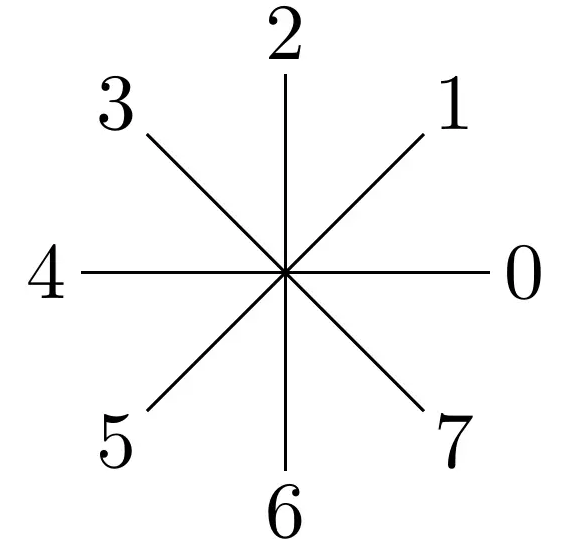
\includegraphics[width=0.2\textwidth]{direction.png}
    \caption{chemfig方向的定义}
    \label{fig:direction}
\end{figure}

举个乙烷的例子:

\begin{center}
  \chemfig{C(-[2]H)(-[4]H)(-[6]H)-C(-[2]H)(-[6]H)-H}
\end{center}

上述乙烷代码如下:
{\verb|\chemfig{C(-[2]H)(-[4]H)(-[6]H)-C(-[2]H)(-[6]H)-H}|}
代码中 (-[X]Y) 内的数字 X 就表示了内容 Y 的位置,其中中括号([ ])的位置通常紧跟在化学键(-、= 等)之后。例如2表示的就是向上的方向,4 表示向左,6 表示向右。

再画一个苯环:
\begin{center}
  \chemfig{*6(-=-=-=)}
\end{center}

%%%%%%%%%%%%%%%%%%%%%%%%%%%%%%%%%%%%%%%%%%%%%%%%%%%%%%

\section{图像布局}
\label{sec.figure}
\subsection{单图布局}

    这是一段随机插入的文本,用来填充模板布局,感受模板视觉效果。这是一段随机插入的文本,用来填充模板布局,感受模板视觉效果。这是一段随机插入的文本,用来填充模板布局,感受模板视觉效果。这是一段随机插入的文本,用来填充模板布局,感受模板视觉效果。这是一段随机插入的文本,用来填充模板布局,感受模板视觉效果。这是一段随机插入的文本,用来填充模板布局,感受模板视觉效果。
    
    这是一段随机插入的文本,用来填充模板布局,感受模板视觉效果。这是一段随机插入的文本,用来填充模板布局,感受模板视觉效果。这是一段随机插入的文本,用来填充模板布局,感受模板视觉效果。这是一段随机插入的文本,用来填充模板布局,感受模板视觉效果。这是一段随机插入的文本,用来填充模板布局,感受模板视觉效果。这是一段随机插入的文本,用来填充模板布局,感受模板视觉效果。

单图布局如图\ref{F.glut_single}所示。

\begin{figure}[hbt]
\centering
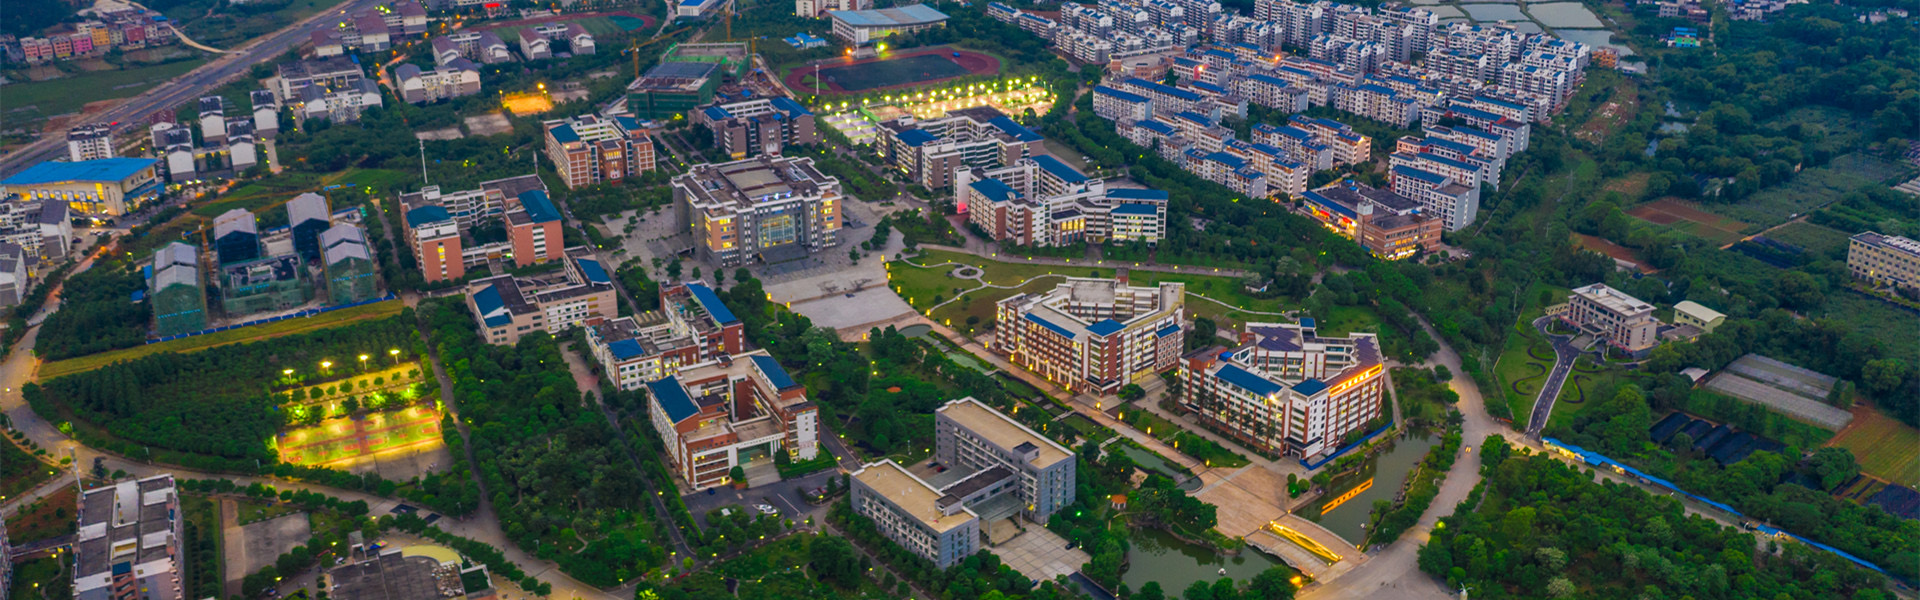
\includegraphics[width=1.0\textwidth]{banner.jpeg}
\caption{单图布局示例}
\label{F.glut_single}
\end{figure}

\subsection{横排布局}

横排布局如图\ref{F.glut_row}所示。

\begin{figure}[!htb]
    \centering
    \begin{subfigure}[t]{0.24\linewidth}
        \begin{minipage}[b]{1\linewidth}
        
\includegraphics[width=1\linewidth]{glut.png}
        \caption{第一张}
        \end{minipage}
    \end{subfigure}
    \begin{subfigure}[t]{0.24\linewidth}
        \begin{minipage}[b]{1\linewidth}
        
\includegraphics[width=1\linewidth]{glut.png}
        \caption{第二张}
        \end{minipage}
    \end{subfigure}
    \caption{横排布局示例}
    \label{F.glut_row}
\end{figure}

    这是一段随机插入的文本,用来填充模板布局,感受模板视觉效果。这是一段随机插入的文本,用来填充模板布局,感受模板视觉效果。这是一段随机插入的文本,用来填充模板布局,感受模板视觉效果。这是一段随机插入的文本,用来填充模板布局,感受模板视觉效果。这是一段随机插入的文本,用来填充模板布局,感受模板视觉效果。这是一段随机插入的文本,用来填充模板布局,感受模板视觉效果。
    
    这是一段随机插入的文本,用来填充模板布局,感受模板视觉效果。这是一段随机插入的文本,用来填充模板布局,感受模板视觉效果。这是一段随机插入的文本,用来填充模板布局,感受模板视觉效果。这是一段随机插入的文本,用来填充模板布局,感受模板视觉效果。这是一段随机插入的文本,用来填充模板布局,感受模板视觉效果。这是一段随机插入的文本,用来填充模板布局,感受模板视觉效果。

\subsection{竖排布局}
竖排布局如图\ref{F.glut_col}所示。

\begin{figure}[!htb]
    \centering
    \begin{subfigure}[t]{0.15\linewidth}
        \captionsetup{justification=centering} %ugly hacks
        \begin{minipage}[b]{1\linewidth}
        
\includegraphics[width=1\linewidth]{glut.png}
        \caption{第一张}
        \end{minipage}
    \end{subfigure}\\
    \begin{subfigure}[t]{0.15\linewidth}
        \captionsetup{justification=centering} %ugly hacks
        \begin{minipage}[b]{1\linewidth}
        
\includegraphics[width=1\linewidth]{glut.png}
        \caption{第二张}
        \end{minipage}
    \end{subfigure}
    \caption{竖排布局示例}
    \label{F.glut_col}
\end{figure}

    这是一段随机插入的文本,用来填充模板布局,感受模板视觉效果。这是一段随机插入的文本,用来填充模板布局,感受模板视觉效果。这是一段随机插入的文本,用来填充模板布局,感受模板视觉效果。这是一段随机插入的文本,用来填充模板布局,感受模板视觉效果。这是一段随机插入的文本,用来填充模板布局,感受模板视觉效果。这是一段随机插入的文本,用来填充模板布局,感受模板视觉效果。
    
    这是一段随机插入的文本,用来填充模板布局,感受模板视觉效果。这是一段随机插入的文本,用来填充模板布局,感受模板视觉效果。这是一段随机插入的文本,用来填充模板布局,感受模板视觉效果。这是一段随机插入的文本,用来填充模板布局,感受模板视觉效果。这是一段随机插入的文本,用来填充模板布局,感受模板视觉效果。这是一段随机插入的文本,用来填充模板布局,感受模板视觉效果。

\subsection{竖排多图横排布局}

\begin{figure}[!htb]
    \centering
    \begin{subfigure}[t]{0.13\linewidth}
        \captionsetup{justification=centering} 
        \begin{minipage}[b]{1\linewidth}
        
\includegraphics[width=1\linewidth]{glut.png} \vspace{-1ex} \vfill
        
\includegraphics[width=1\linewidth]{glut.png}
        \caption{第一张}
        \end{minipage}
    \end{subfigure}
    \begin{subfigure}[t]{0.13\linewidth}
        \captionsetup{justification=centering} 
        \begin{minipage}[b]{1\linewidth}
        
\includegraphics[width=1\linewidth]{glut.png} \vspace{-1ex} \vfill
        
\includegraphics[width=1\linewidth]{glut.png}
        \caption{第二张}
        \end{minipage}
    \end{subfigure}
    \caption{竖排多图横排布局}
    \label{F.glut_col_row}
\end{figure}

竖排多图横排布局如图\ref{F.glut_col_row}所示。注意看(a)、(b)编号与图关系。


\subsection{横排多图竖排布局}

    这是一段随机插入的文本,用来填充模板布局,感受模板视觉效果。这是一段随机插入的文本,用来填充模板布局,感受模板视觉效果。这是一段随机插入的文本,用来填充模板布局,感受模板视觉效果。这是一段随机插入的文本,用来填充模板布局,感受模板视觉效果。这是一段随机插入的文本,用来填充模板布局,感受模板视觉效果。这是一段随机插入的文本,用来填充模板布局,感受模板视觉效果。

\begin{figure}[!htb]
    \centering
    \begin{subfigure}[t]{0.3\linewidth}
        \captionsetup{justification=centering} 
        \begin{minipage}[b]{1\linewidth}
        
\includegraphics[width=0.45\linewidth]{glut.png}
        
\includegraphics[width=0.45\linewidth]{glut.png}
        \caption{}
        \end{minipage}
    \end{subfigure}\\
    \begin{subfigure}[t]{0.3\linewidth}
        \captionsetup{justification=centering} 
        \begin{minipage}[b]{1\linewidth}
        
\includegraphics[width=0.45\linewidth]{glut.png}
        
\includegraphics[width=0.45\linewidth]{glut.png}
        \caption{}
        \end{minipage}
    \end{subfigure}
    \caption{横排多图竖排布局}
    \label{F.glut_row_col}
\end{figure}

横排多图竖排布局如图\ref{F.glut_row_col}所示。注意看(a)、(b)编号与图关系。

\newpage
%%%%%%%%%%%%%%%%%%%%%%%%%%%%%%%%%%%%%%%%%%%%%%%%%%%%%%%

\section{表格插入示例}
表格如表\ref{T.example}所示,latex表格技巧很多,这里不再详细介绍。

\begin{table}[htb]
  \centering
  \caption{按照学术论文的一般规范,表格为三线表。}
  \label{T.example}
  \begin{tabular}{ccccc}
\toprule
A   &  B  &  C  & D  & E \\
\midrule
1 	& 一 & 壹 & one 	 & 啊\\
2 	& 二 & 贰 & two 	 & 哈\\
3 	& 三 & 叁 & three & 嗯\\
4 	& 四 & 肆 & four	 & 嘿\\
\bottomrule
\end{tabular}
\end{table}

\newpage

%%%%%%%%%%%%%%%%%%%%%%%%%%%%%%%%%%%%%%%%%%%%%%%%%%%%%%
\section{参考文献插入示例}

LaTeX\cite{lamport1994latex}插入参考文献最方便的方式是使用bibliography\cite{hu2020},大多数出版商的论文页面\cite{lamport1994latex}都会有导出bib格式参考文献的链接,把每个文献的bib放入``GLUTthesis.bib'',然后用bibkey即可插入参考文献。

\newpage
%%%%%%%%%%%%%%%%%%%%%%%%%%%%%%%%%%%%%%%%%%%%%%%%%%%%%%
\section{总结与展望}

XX的XX都存在XX,所以我们XX,本章总结XX。

\subsection{本文工作总结}
在总结和分析已有XX的理论基础上,本文对XX进行了XX,主要工作如下:

%手工编号
(1)图片插入布局,如第\ref{sec.figure}章所示。

(2)XXXXXXXXXX

(3)XXXXXXXXXX

(4)XXXXXXXXXX


\subsection{工作展望}
本课题针对XX,鉴于XXX,对XX进行了提高,但是XXX,所以有如下XX:

(1)目前XX虽然XX,但是XX仍然XX,所以XX仍然是一个值得XX的问题。

(2)随着XX,XX具有XX的问题,仍值得进一步XX。

(3)本课题在XX有了XX,但是XX的XX还存在XX,所以XX。

\newpage
